\documentclass[a4paper,10pt]{article}
\usepackage{graphicx}
\usepackage[russian]{babel}
\usepackage{cmap}
\usepackage[T2A]{fontenc}
\usepackage[utf8]{inputenc}
\usepackage{mathtools}
\usepackage{float}
\usepackage{titlesec}
\usepackage{varioref}
\usepackage{fancyhdr}
\usepackage{multicol}
\usepackage{mathrsfs}
\usepackage{wrapfig}
\usepackage{gensymb}
\usepackage{subcaption}
\usepackage[table]{xcolor}
\usepackage{amsmath}

\begin{document}

\begin{center}
    {\large МОСКОВСКИЙ ФИЗИКО-ТЕХНИЧЕСКИЙ ИНСТИТУТ (НАЦИОНАЛЬНЫЙ ИССЛЕДОВАТЕЛЬСКИЙ УНИВЕРСИТЕТ)}
\end{center}

\vspace{4.5cm}
{\Large
\begin{center}
\end{center}
{\bf Отчёт о выполнении лабораторной работы 3.3.5}\\
Эффект Холла в металлах
}
\vspace{2cm}
\begin{flushright}
    {\normalsize Галкина Мария, Высоцкая Ирина \\
    \vspace{0.2cm}
    Б03-502}
\end{flushright}
\vspace{8cm}


\section{Аннотация}
\noindent \textbf{Цель работы:} измерение подвижности и концентрации носителей
заряда в металлах\\
\textbf{В работе используются:} электромагнит с источником питания, источник
постоянного тока, микровольтметр, амперметры, цифровой магнитометр, образцы
из меди, серебра и цинка

\section{Теоретические сведения}
Одновременное исследование эффекта Холла и проводимости позволяет находить плотность носителей заряда и их подвижность. Суть эффекта Холла состоит в следующем. Пусть через однородную пластину металла вдоль оси \(x\) течет ток \(I\). Если эту пластину поместить в магнитное поле, направленное по оси \(y\), то между гранями появится разность потенциалов. На электрон, движущийся со скоростью \(\mathbf{v}\) в электромагнитном поле, действует сила Лоренца.
\[
\mathbf{F}_\text{л} = -e\mathbf{E} - e\mathbf{v} \times \mathbf{B}
\]

В нашем случае сила, обусловленная вторым слагаемым, направлена вдоль оси \(z\).
\[
F_B = e |v_x| B
\]

Под действием этой силы электроны отклоняются к грани Б, заряжая ее отрицательно. При этом на грани А накапливаются нескомпенсированные положительные заряды, что приводит к возникновению электрического поля \(E_z\), направленного от А к Б, которое действует на электроны силой \(F_E = eE_z\), направленной против силы \(F_B\). В стационарном режиме \(F_E\) уравновешивает \(F_B\), и накопление зарядов на боковых гранях прекращается. Из условия равновесия найдем:
\[
E_z = |v_x| B
\]

С полем \(E_z\) связана разность потенциалов \(U_\text{АБ}\) между гранями А и Б.
\[
U_\text{АБ} = -E_z l = -|v_x| Bl
\]

Заметим, что сила тока
\[
I = ne|v_x| l \cdot a,
\]

отсюда найдем ЭДС Холла:
\[
U_x = U_\text{АБ} = -\frac{IB}{nea} = -R_x \cdot \frac{IB}{a},
\]
где \(R_x = \frac{1}{ne}\) -- постоянная Холла.\\

\noindent \textbf{Экспериментальная установка}\\
\begin{center}
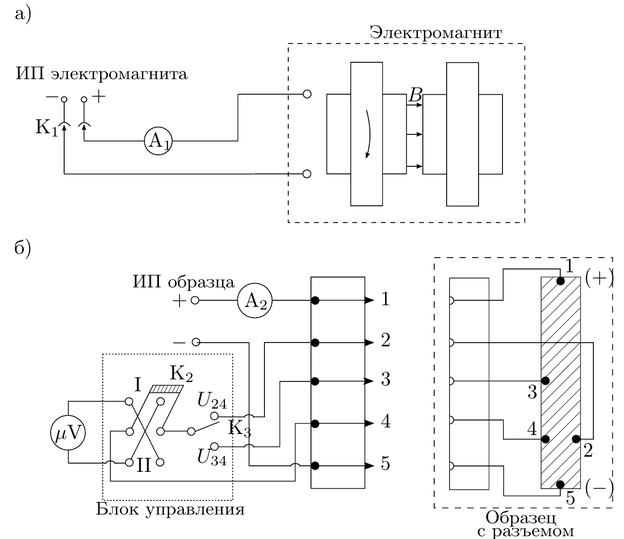
\includegraphics[width=10cm]{ust.png}
\end{center}
В зазоре электромагнита создается постоянное магнитное поле, которое можно регулировать с помощью источника питания электромагнита.
Иногда контакты 2 и 4 вследствие неточности подпайки не лежат на одной эквипотенциали, и тогда напряжение между ними связано не только с эффектом Холла, но и с омическим напряжением, вызванным протеканием основного тока через образец.
Неточности измерений можно избежать путем фиксирования этого омического напряжения при нулевом значении силы тока и отсчитывания от него Холловского напряжения.
\[
\varepsilon_x = U_{24} \pm U_0
\]

Измерив ток в образце и напряжение \(U_{34}\) между контактами 3 и 4 в отсутствии магнитного поля, можно, зная параметры образца, рассчитать проводимость материала образца по очевидной формуле:
\[
\sigma = \frac{I l}{U_{34} a l}
\]

\section{Экспериментальные данные и обработка результатов}
Проведём градуировку: измерим зависимость $B(I_M)$ и построим её график для
получения градуировочного коэффициента
\begin{center}
\begin{tabular}{|c|c|c|}
	\hline
	$I_M$, A & $B$, мТл & $\sigma_B$, мТл\\ \hline
	0.00 & 18.82 & 0.01\\
	0.15 & 182.2 & 0.1\\
	0.30 & 360 & 1\\
	0.45 & 522 & 1\\
	0.60 & 689 & 1\\
	0.75 & 844 & 1\\
	0.90 & 937 & 1\\
	1.05 & 1014 & 1\\ \hline
\end{tabular}\\
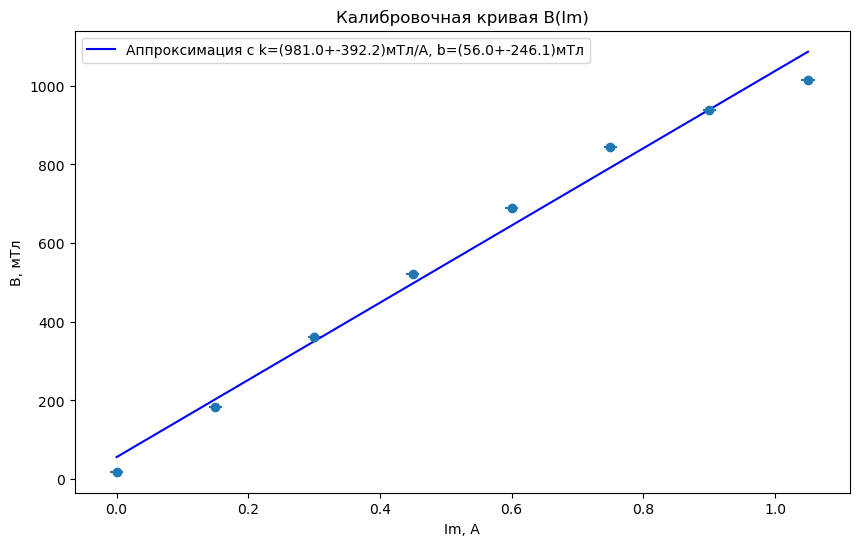
\includegraphics[width=15cm]{cal.png}
\end{center}

Рассчитаем и построим графики ЭДС Холла как функции $\varepsilon_x(B)$ для
разных значений тока I через образец меди (шкала микровольтметра: 3мкв=75дел):\\
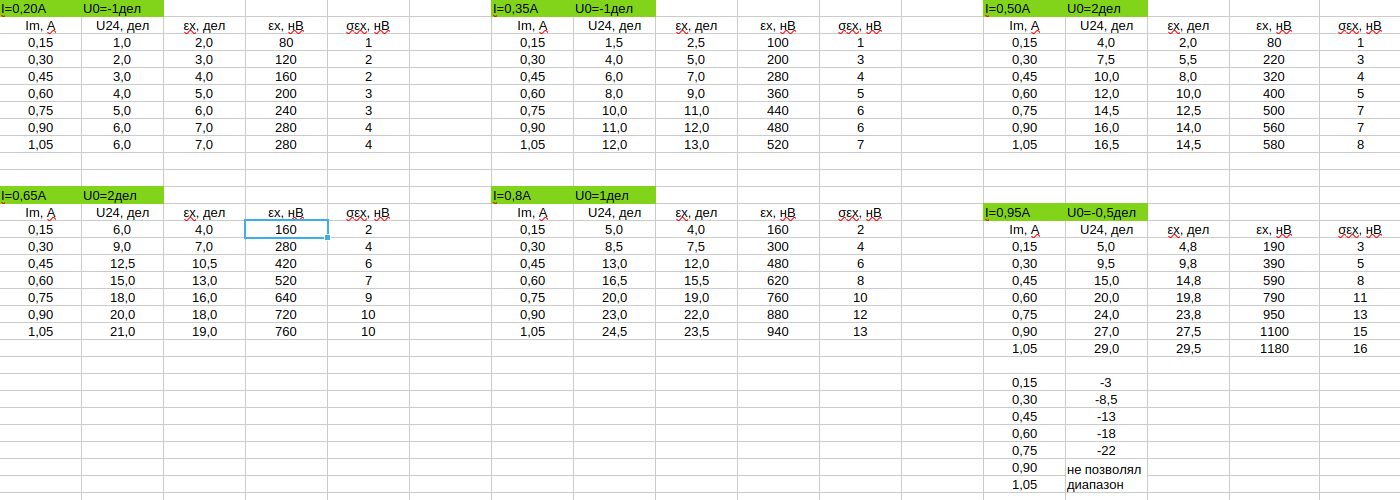
\includegraphics[width=16cm]{tables.png}\\
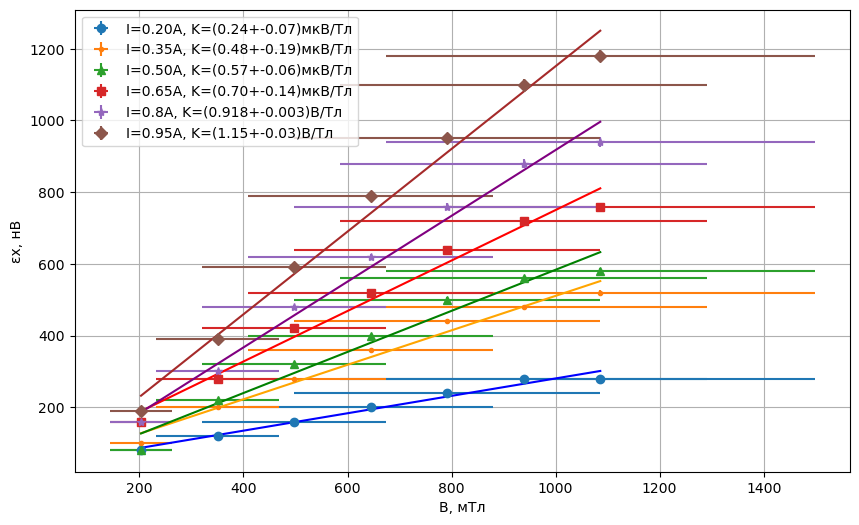
\includegraphics[width=15cm]{zhopa.png}\\
Для определения постоянной Холла $R_x$ построим график $K(I)$ и посчитаем его
коэффициент наклона:
\begin{center}
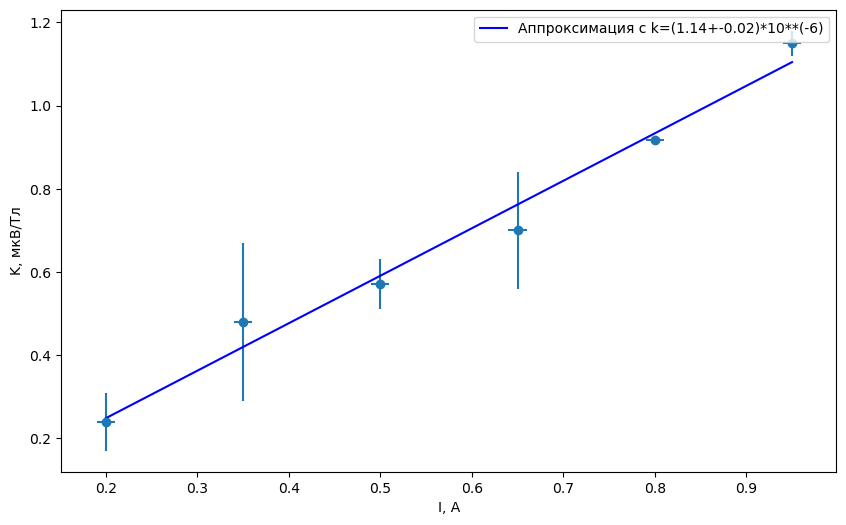
\includegraphics[width=10cm]{nice_graph.png}
\end{center}
\textbf{Параметры меди}:\hspace{1cm} $L_{3, 4}=6\text{мм} \hspace{1cm} a=0.05\text{мм} \hspace{1cm}
l=8\text{мм}$\\
Отсюда постоянная Холла $R_x = -K\cdot a = -(5.7\pm0.1)\cdot10^{-11}
\frac{\text{м}^3}{\text{Кл}}$ \\
$R_x^{\text{теор}} = -5.5\cdot10^{-11}\frac{\text{м}^3}{\text{Кл}}$\\
В пределах погрешности наше значение не совпадает с теоретическим, разница
составила 3.5\% \\

Теперь найдём значение постоянную Холла для цинка по примерно такому же
алгоритму:\\
Таблица с расчётом ЭДС Холла (диапазон измерений микровольтметром был
3мкв=75дел):
\begin{center}
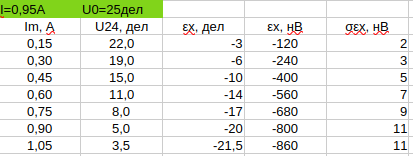
\includegraphics[width=7cm]{table.png}\\
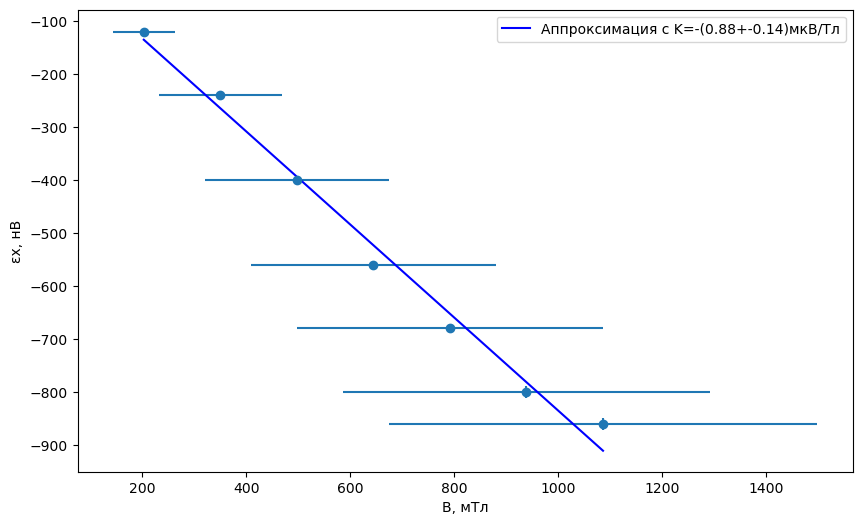
\includegraphics[width=15cm]{ne_zhopa.png}
\end{center}
\textbf{Параметры цинка:}\hspace{1cm}$L_{3, 4}=4\text{мм} \hspace{1cm} a=0.08\text{мм} \hspace{1cm}
l=10\text{мм}$\\
$R_x = -\frac{K\cdot a}{I} = (0.74\pm0.11) \frac{\text{м}^3}{\text{Кл}}$,
\hspace{1cm} $R_x^{\text{теор}} = 0.55\frac{\text{м}^3}{\text{Кл}}$\\
В пределах погрешности экспериментальное значение не совпадает с теоретическим,
разница составляет 13\%






\subsection*{Удельная проводимость \(\sigma\)}
Формула: \(\sigma = \frac{I \cdot L_{34}}{U_{34} \cdot a \cdot l}\), где \(I = 1\) А, \(\Delta I = 0.01\) А, \(\Delta U_{34} = 5 \cdot 10^{-6}\) В, \(\Delta L_{34} = \Delta l = 0.01\) мм.
\\
Относительная погрешность: \(\frac{\Delta \sigma}{\sigma} = \sqrt{(\frac{\Delta I}{I})^2 + (\frac{\Delta U}{U})^2 + (\frac{\Delta L}{L})^2 + (\frac{\Delta a}{a})^2 + (\frac{\Delta l}{l})^2}\).
\\
\begin{itemize}
    \item \textbf{Медь:} \(\sigma_{Cu} = 5.0 \cdot 10^7 \, \text{Ом}^{-1}\text{м}^{-1}\). 
    \(\frac{\Delta \sigma_{Cu}}{\sigma_{Cu}} \approx 20.1\%\), откуда \(\Delta \sigma_{Cu} = 1.0 \cdot 10^7 \, \text{Ом}^{-1}\text{м}^{-1}\).
    \item \textbf{Цинк:} \(\sigma_{Zn} = 1.52 \cdot 10^7 \, \text{Ом}^{-1}\text{м}^{-1}\). 
    \(\frac{\Delta \sigma_{Zn}}{\sigma_{Zn}} \approx 20.2\%\), откуда \(\Delta \sigma_{Zn} = 0.3 \cdot 10^7 \, \text{Ом}^{-1}\text{м}^{-1}\).
\end{itemize}
Полученные значения хорошо согласуются со справочными данными (для меди \(\sim 5.9 \cdot 10^7\), для цинка \(\sim 1.6 \cdot 10^7\)).

\subsection*{Концентрация носителей заряда \(n\)}
Формула: \(n = \frac{1}{R_x \cdot e}\), где \(e = 1.6 \cdot 10^{-19}\) Кл. 
Погрешность: \(\frac{\Delta n}{n} = \frac{\Delta R_x}{R_x}\).
\begin{itemize}
    \item \textbf{Медь:} \(n_{Cu} = 1.1 \cdot 10^{23} \, \text{см}^{-3}\). 
    \(\frac{\Delta n_{Cu}}{n_{Cu}} \approx 1.75\%\), откуда \(\Delta n_{Cu} \approx 0.02 \cdot 10^{23} \, \text{см}^{-3}\).
    \item \textbf{Цинк:} \(n_{Zn} = 8.4 \cdot 10^{22} \, \text{см}^{-3}\). 
    \(\frac{\Delta n_{Zn}}{n_{Zn}} \approx 14.8\%\), откуда \(\Delta n_{Zn} \approx 1.2 \cdot 10^{22} \, \text{см}^{-3}\). 
\end{itemize}

\subsection*{Подвижность носителей заряда \(b\)}
Формула: \(b = \sigma \cdot R_x\). 
Погрешность: \(\frac{\Delta b}{b} = \sqrt{(\frac{\Delta \sigma}{\sigma})^2 + (\frac{\Delta R_x}{R_x})^2}\).
\begin{itemize}
    \item \textbf{Медь:} \(b_{Cu} = 5.0 \cdot 10^7 \cdot 5.7 \cdot 10^{-11} = 28.5 \, \text{см}^2/(\text{В}\cdot\text{с})\). 
    \(\frac{\Delta b_{Cu}}{b_{Cu}} \approx 20.2\%\), откуда \(\Delta b_{Cu} \approx 5.8 \, \text{см}^2/(\text{В}\cdot\text{с})\).
    \item \textbf{Цинк:} \(b_{Zn} = 1.52 \cdot 10^7 \cdot 0.74 \cdot 10^{-10} = 11.2 \, \text{см}^2/(\text{В}\cdot\text{с})\). 
    \(\frac{\Delta b_{Zn}}{b_{Zn}} \approx 25.0\%\), откуда \(\Delta b_{Zn} \approx 2.8 \, \text{см}^2/(\text{В}\cdot\text{с})\).
\end{itemize}

\subsection*{Сводная таблица результатов}
\begin{center}
\resizebox{\textwidth}{!}{%
\begin{tabular}{|c|c|c|c|c|c|c|}
    \hline
    Металл & \(R_x \pm \Delta R_x\), \(10^{-11} \frac{\text{м}^3}{\text{Кл}}\) & Табл. \(R\), \(10^{-11} \frac{\text{м}^3}{\text{Кл}}\) & Знак носителей & \(n \pm \Delta n\), \(10^{23} \, \text{см}^{-3}\) & \(\sigma \pm \Delta \sigma\), \(10^7 \, (\text{Ом}\cdot\text{м})^{-1}\) & \(b \pm \Delta b\), \(\frac{\text{см}^2}{\text{В}\cdot\text{с}}\) \\ \hline
    Медь & \(-(5.7 \pm 0.1)\) & \(-5.5\) & \(-\) & \(1.1 \pm 0.02\) & \(5.0 \pm 1.0\) & \(28.5 \pm 5.8\) \\ \hline
    Цинк & \((0.74 \pm 0.11) \cdot 10^{-10}\) & \(0.55 \cdot 10^{-10}\) & \(+\) & \(0.84 \pm 0.12\) & \(1.5 \pm 0.3\) & \(11.2 \pm 2.8\) \\ \hline
\end{tabular}%
}
\end{center}

\section*{Вывод}
В ходе работы был исследован эффект Холла в металлах. Определены постоянные Холла для меди и цинка. Рассчитаны концентрации и подвижности носителей заряда, а также удельные проводимости образцов. Полученные экспериментальные значения \(R_x\) имеют отклонения от табличных (для меди 3.5\%, для цинка 13\%), что может быть связано с погрешностями измерений и неточностью геометрических параметров образцов. Значения удельной проводимости хорошо согласуются со справочными данными.












\end{document}